\documentclass[11pt,a4paper]{article}

\usepackage[utf8]{inputenc}
\usepackage[T1]{fontenc}
\usepackage{geometry}
\geometry{margin=2.5cm,headheight=14pt}
\usepackage{listings}
\usepackage{xcolor}
\usepackage{graphicx}
\usepackage{hyperref}
\usepackage{enumitem}
\usepackage{booktabs}
\usepackage{fancyhdr}
\usepackage{titlesec}
\usepackage{amsmath}

\hypersetup{
    colorlinks=true,
    linkcolor=blue,
    urlcolor=blue,
    citecolor=blue
}

% ---------- estilo de código ----------
\definecolor{codebg}{RGB}{245,245,245}
\definecolor{codegreen}{RGB}{0,128,0}
\definecolor{codegray}{RGB}{120,120,120}
\definecolor{codeblue}{RGB}{0,0,180}

\lstdefinestyle{codestyle}{
    backgroundcolor=\color{codebg},
    commentstyle=\color{codegreen},
    keywordstyle=\color{codeblue}\bfseries,
    numberstyle=\tiny\color{codegray},
    stringstyle=\color{codegreen},
    basicstyle=\ttfamily\footnotesize,
    breakatwhitespace=false,
    breaklines=true,
    captionpos=b,
    keepspaces=true,
    numbers=left,
    numbersep=6pt,
    showspaces=false,
    showstringspaces=false,
    showtabs=false,
    tabsize=2,
    frame=single,
    rulecolor=\color{black!20}
}
\lstset{style=codestyle}
\lstdefinelanguage{ini}{
   basicstyle=\ttfamily\footnotesize,
   morecomment=[l]{;},
   morecomment=[l]{\#}
}

\pagestyle{fancy}
\fancyhf{}
\fancyhead[L]{Proyecto Sensor de pH}
\fancyhead[R]{\thepage}
\renewcommand{\headrulewidth}{0.4pt}

\title{
    \Large \textbf{Documentación Técnica} \\
    \large Sistema de Monitoreo de pH del Agua con ESP32 y Dashboard Web
}
\author{Daniela Romero y Débora Vizama}
\date{\today}

\begin{document}

\maketitle
\thispagestyle{empty}
\tableofcontents
\newpage

% ======================================================
\section{Introducción}

Este documento describe el diseño, los componentes de hardware y el
funcionamiento del software del sistema de monitoreo de pH del agua
desarrollado para el proyecto de feria científica. El objetivo del
sistema es permitir que los estudiantes viertan una muestra de agua
(destilada, con sal, con tierra, con limón, etc.) y observen en tiempo
real, a través de un dashboard web, cómo cambian el pH y la
temperatura, junto con una alerta visual tipo semáforo que indica si
el agua se encuentra en un estado seguro, marginal o contaminado.

El sistema se compone de tres partes:

\begin{enumerate}
    \item \textbf{Hardware}: microcontrolador ESP32 conectado a un
    sensor de pH industrial (protocolo RS-485) y a un sensor de
    temperatura sumergible (protocolo OneWire).
    \item \textbf{Software de adquisición}: un programa embebido en
    el ESP32 que lee los sensores y los imprime por el puerto serial
    (USB), y un script en Python en la computadora que traduce esa
    información y la envía a un servidor.
    \item \textbf{Software de visualización}: un servidor backend
    (Flask) que almacena las lecturas, y un dashboard web
    (Streamlit) que las muestra en gráficos dinámicos y alertas de
    color.
\end{enumerate}

% ======================================================
\section{Componentes de Hardware Utilizados}

\begin{table}[h]
\centering
\begin{tabular}{@{}p{4cm}p{9cm}@{}}
\toprule
\textbf{Componente} & \textbf{Descripción / Función} \\
\midrule
ESP32 (WROOM-32) &
Microcontrolador principal. Se encarga de comunicarse con el sensor
de pH por protocolo Modbus RS-485, leer el sensor de temperatura por
OneWire, e imprimir los resultados por el puerto Serial (USB) hacia
la computadora. \\
\addlinespace
Sensor de pH industrial (RS-485) &
Sensor sumergible con salida digital sobre RS-485 (protocolo
Modbus). Entrega el valor de pH multiplicado por 10 en un registro
que se lee mediante una trama de comando fija. \\
\addlinespace
Interfaz conversora RS-232/RS-485 &
Módulo intermedio que adapta las señales del ESP32 (nivel TTL) al
estándar eléctrico RS-485 que requiere el sensor de pH industrial. \\
\addlinespace
Sensor de temperatura (DS18B20, OneWire) &
Sensor sumergible de temperatura, conectado por el protocolo
OneWire a un pin digital del ESP32 (pin 27 en este proyecto). \\
\addlinespace
Transformador / fuente de alimentación 12V 2A &
Fuente de poder externa que alimenta al sensor de pH y a la interfaz
RS-485, ya que estos componentes requieren 12V, un voltaje mayor al
que puede entregar el propio ESP32 (que trabaja a 3.3V/5V). \\
\addlinespace
Cable USB &
Utilizado para alimentar y programar el ESP32, y además como canal
de comunicación serial (Serial Monitor) hacia la computadora, por
donde se transmiten las lecturas de pH y temperatura que luego
recoge el script \texttt{serial\_reader.py}. \\
\addlinespace
Computadora (laptop) &
Ejecuta el backend (Flask), el script de lectura serial y el
dashboard (Streamlit). \\
\bottomrule
\end{tabular}
\caption{Componentes de hardware del sistema}
\end{table}

\subsection{Diagrama de conexión}

\begin{figure}[h]
\centering
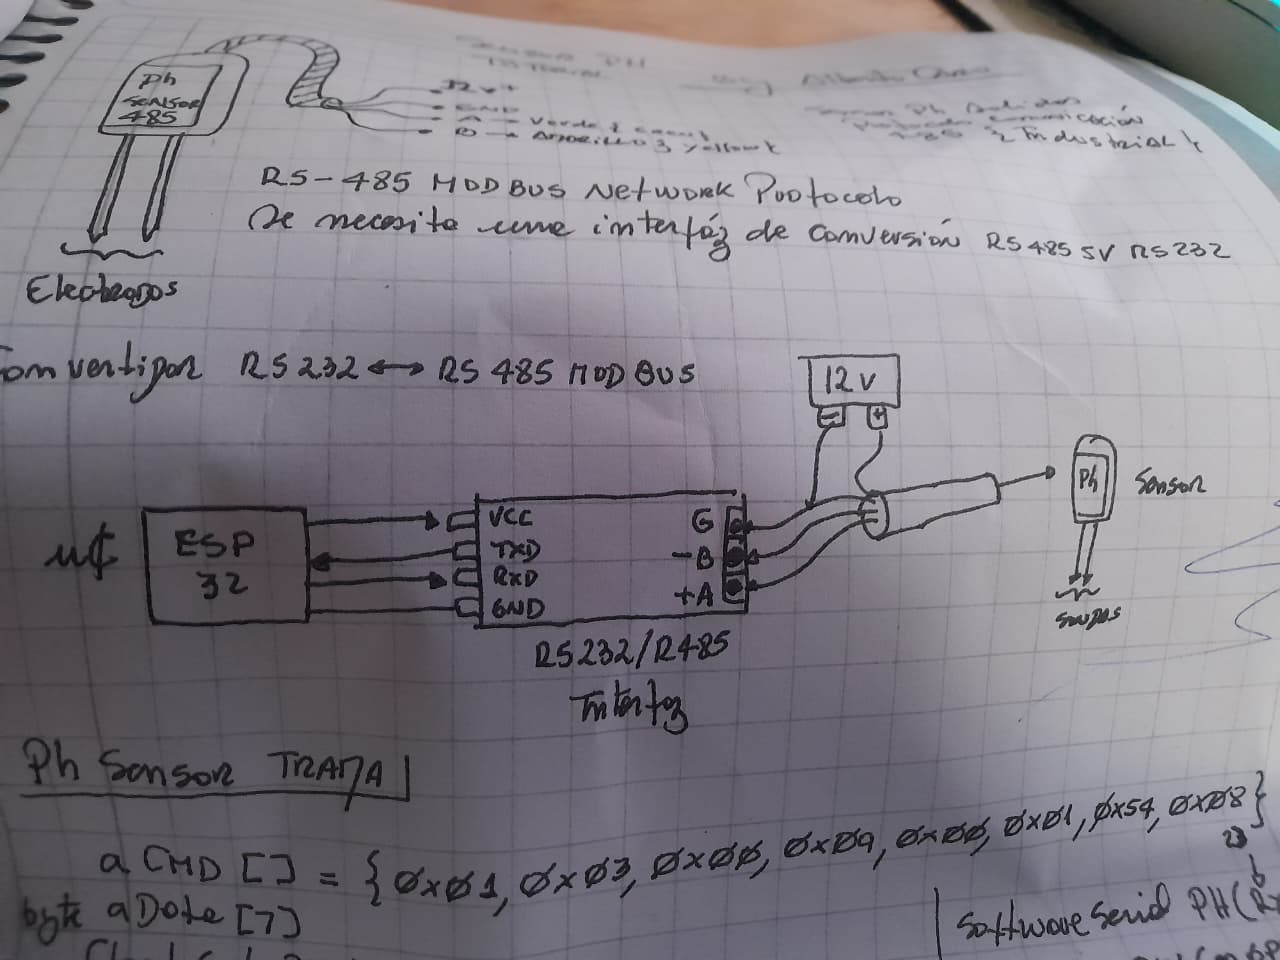
\includegraphics[width=0.95\textwidth]{diagrama_conexion.jpeg}
\caption{Diagrama de conexión del sensor de pH: ESP32, interfaz de
conversión RS-232/RS-485, sensor de pH y fuente de 12V. Elaborado a
partir de las notas originales del tutorial del sensor.}
\end{figure}

\textit{Nota:} el sensor de pH y la interfaz RS-485 requieren
alimentación de 12V, provista por el transformador. El ESP32 se
alimenta de forma independiente por el cable USB conectado a la
computadora, lo que además permite la transmisión de datos por
puerto serial sin necesidad de una red WiFi.

% ======================================================
\section{Arquitectura del Software}

El sistema sigue un flujo de datos lineal, sin necesidad de conexión
a una red WiFi, ya que toda la comunicación entre el ESP32 y la
computadora ocurre a través del mismo cable USB:

\begin{center}
\begin{verbatim}
ESP32 (lee sensores)
   --> Serial/USB -->
serial_reader.py (lee el puerto y reenvía)
   --> HTTP POST (JSON) -->
app.py / Flask (guarda en SQLite, expone API)
   <-- HTTP GET (JSON) --
streamlit_app.py (dashboard: gráficos y semáforo)
\end{verbatim}
\end{center}

Esta arquitectura desacopla la adquisición de datos (hardware) de la
visualización (dashboard), lo que permite, por ejemplo, generar datos
de prueba sin el sensor físico (ver \texttt{simulate\_data.py}),
o eventualmente reemplazar el mecanismo de transporte (por ejemplo,
migrar a WiFi/MQTT) sin modificar el dashboard.

% ======================================================
\section{Explicación de los Códigos, Método por Método}

\subsection{\texttt{esp32/esp32\_ph\_sensor.ino}}

Código embebido que corre directamente en el microcontrolador ESP32.
Es responsable de leer los dos sensores físicos y reportar los
valores por el puerto serial.

\begin{lstlisting}[language=C++,caption={Declaraciones y variables globales}]
#include <OneWire.h>
#include <DallasTemperature.h>
#define nRx 23
#define nTx 22
const byte aCMD[] = {0x01,0x03,0x00,0x09,0x00,0x01,0x54,0x08};
const byte nGPTE = 27;
byte aData[7];
float fPH, fTE;
OneWire oneWire(nGPTE);
DallasTemperature st(&oneWire);
HardwareSerial PHS(2);
\end{lstlisting}

\textbf{Explicación:}
\begin{itemize}
    \item \texttt{aCMD[]}: trama de comando Modbus fija que se envía
    al sensor de pH para solicitar la lectura de su registro
    interno. Sigue el protocolo Modbus RTU: dirección de esclavo,
    función, dirección de registro y CRC.
    \item \texttt{nGPTE = 27}: pin digital del ESP32 donde está
    conectado el sensor de temperatura OneWire.
    \item \texttt{PHS = HardwareSerial(2)}: se utiliza el segundo
    puerto serial de hardware del ESP32 (distinto del puerto USB de
    depuración) para comunicarse con la interfaz RS-485.
    \item \texttt{fPH}, \texttt{fTE}: variables donde se almacenan
    los últimos valores leídos de pH y temperatura.
\end{itemize}

\begin{lstlisting}[language=C++,caption={Método setup()}]
void setup() {
  Serial.begin(9600);
  PHS.begin(9600, SERIAL_8N1, nRx, nTx);
  st.begin();
  delay(3000);
}
\end{lstlisting}

\textbf{Explicación:} inicializa el puerto Serial de depuración (el
que verá la computadora por USB), inicializa el puerto Serial hacia
la interfaz RS-485 con los parámetros de comunicación del sensor de
pH (9600 baudios, 8 bits de datos, sin paridad, 1 bit de parada), e
inicializa la librería del sensor de temperatura OneWire. El
\texttt{delay(3000)} da tiempo a que los periféricos se estabilicen
antes de comenzar a leer.

\begin{lstlisting}[language=C++,caption={Método loop() - lectura de pH}]
void loop() {
  PHS.flush();
  if (PHS.write(aCMD, sizeof(aCMD)) == 8) {
    PHS.readBytes(aData, 7);
  }
  fPH = aData[4] / 10.0;
  Serial.print("Soil PH: ");
  Serial.println(fPH, 1);
  ...
\end{lstlisting}

\textbf{Explicación:} se envía la trama de comando \texttt{aCMD} al
sensor de pH. Si la escritura fue exitosa (8 bytes enviados), se
leen los 7 bytes de respuesta del sensor en el arreglo
\texttt{aData}. El byte en la posición \texttt{aData[4]} contiene el
valor de pH multiplicado por 10 (según la hoja de datos del sensor),
por lo que se divide por 10.0 para obtener el valor real (por
ejemplo, un valor crudo de 71 corresponde a pH 7.1). El resultado se
imprime por el puerto Serial en un formato de texto fijo
(\texttt{"Soil PH: X.X"}), que luego será interpretado por el script
de Python.

\begin{lstlisting}[language=C++,caption={Método loop() - lectura de temperatura}]
  st.requestTemperatures();
  fTE = st.getTempCByIndex(0);
  Serial.print("Temperatura: ");
  Serial.print(fTE);
  Serial.println(" grados C");
  delay(10000);
}
\end{lstlisting}

\textbf{Explicación:} se solicita al sensor OneWire una nueva
conversión de temperatura (\texttt{requestTemperatures()}) y se lee
el resultado del primer sensor detectado en el bus
(\texttt{getTempCByIndex(0)}). El valor se imprime de la misma forma
que el pH, en texto plano por el puerto Serial. El
\texttt{delay(10000)} espacía las lecturas cada 10 segundos.

\subsection{\texttt{backend/serial\_reader.py}}

Script en Python que corre en la computadora. Actúa como puente
entre el puerto USB (donde el ESP32 imprime texto) y el servidor
backend (que espera datos en formato JSON vía HTTP).

\begin{lstlisting}[language=Python,caption={listar\_puertos()}]
def listar_puertos():
    puertos = serial.tools.list_ports.comports()
    for p in puertos:
        print(f"  {p.device}  -  {p.description}")
\end{lstlisting}

\textbf{Explicación:} utiliza la librería \texttt{pyserial} para
listar todos los puertos seriales disponibles en el sistema
operativo (por ejemplo \texttt{COM3} en Windows), junto con una
descripción del dispositivo. Permite al usuario identificar a qué
puerto está conectado el ESP32 antes de iniciar la lectura.

\begin{lstlisting}[language=Python,caption={leer\_y\_enviar(puerto) - núcleo del script}]
def leer_y_enviar(puerto: str):
    with serial.Serial(puerto, BAUDRATE, timeout=2) as ser:
        while True:
            linea = ser.readline().decode("utf-8", errors="ignore").strip()
            match_ph = re.search(r"Soil PH:\s*([\d.]+)", linea)
            match_temp = re.search(r"Temperatura:\s*([\d.]+)", linea)
            if match_ph:
                ph_actual = float(match_ph.group(1))
            if match_temp:
                temp_actual = float(match_temp.group(1))
            if ph_actual is not None and temp_actual is not None:
                enviar_al_backend(ph_actual, temp_actual)
\end{lstlisting}

\textbf{Explicación:} abre una conexión al puerto serial indicado
con la misma velocidad (baudrate) configurada en el ESP32
(9600). En un bucle infinito, lee línea por línea el texto que
imprime el ESP32. Utiliza expresiones regulares
(\texttt{re.search}) para extraer el número que sigue a
\texttt{"Soil PH:"} o a \texttt{"Temperatura:"}. Como el ESP32
imprime ambos valores en líneas separadas dentro del mismo ciclo de
\texttt{loop()}, el script acumula ambos valores y, recién cuando
tiene el par completo, lo envía al backend, reiniciando luego las
variables para esperar el siguiente ciclo.

\begin{lstlisting}[language=Python,caption={enviar\_al\_backend(ph, temp)}]
def enviar_al_backend(ph: float, temp: float):
    r = requests.post(
        BACKEND_URL,
        json={"ph": ph, "temperatura": temp},
        timeout=3,
    )
\end{lstlisting}

\textbf{Explicación:} realiza una petición HTTP \texttt{POST} al
backend Flask, enviando los datos codificados en formato JSON. Este
es el punto de integración entre el mundo del hardware (serial) y el
mundo del dashboard web (HTTP).

\subsection{\texttt{backend/app.py}}

Servidor backend construido con el microframework Flask. Su
responsabilidad es recibir, almacenar y exponer las lecturas de los
sensores.

\begin{lstlisting}[language=Python,caption={init\_db()}]
def init_db():
    conn = sqlite3.connect(DB_PATH)
    conn.execute("""
        CREATE TABLE IF NOT EXISTS lecturas (
            id INTEGER PRIMARY KEY AUTOINCREMENT,
            ph REAL NOT NULL,
            temperatura REAL,
            timestamp TEXT NOT NULL
        )
    """)
    conn.commit()
    conn.close()
\end{lstlisting}

\textbf{Explicación:} crea (si no existe) una base de datos SQLite
local con una tabla \texttt{lecturas}, que almacena cada lectura con
un identificador autoincremental, el valor de pH, la temperatura y
la marca de tiempo en que fue recibida. SQLite se eligió por ser un
motor de base de datos embebido, que no requiere instalar ni
configurar un servidor de base de datos externo.

\begin{lstlisting}[language=Python,caption={recibir\_lectura() - endpoint POST /api/lectura}]
@app.route("/api/lectura", methods=["POST"])
def recibir_lectura():
    data = request.get_json(force=True, silent=True)
    if not data or "ph" not in data:
        return jsonify({"error": "falta el campo 'ph'"}), 400
    ph = float(data["ph"])
    temperatura = float(data.get("temperatura", 0))
    timestamp = datetime.now().isoformat()
    conn.execute("INSERT INTO lecturas (ph, temperatura, timestamp) VALUES (?, ?, ?)", ...)
\end{lstlisting}

\textbf{Explicación:} define el punto de entrada HTTP que recibe
los datos enviados por \texttt{serial\_reader.py} (o por
\texttt{simulate\_data.py}). Valida que el campo \texttt{ph} esté
presente; de lo contrario responde con un error HTTP 400. Si los
datos son válidos, genera una marca de tiempo con el instante actual
del servidor y guarda el registro completo en la base de datos.

\begin{lstlisting}[language=Python,caption={obtener\_lecturas() - endpoint GET /api/lecturas}]
@app.route("/api/lecturas", methods=["GET"])
def obtener_lecturas():
    limite = int(request.args.get("limite", 100))
    filas = conn.execute(
        "SELECT ph, temperatura, timestamp FROM lecturas ORDER BY id DESC LIMIT ?",
        (limite,),
    ).fetchall()
    lecturas = [dict(f) for f in reversed(filas)]
    return jsonify(lecturas)
\end{lstlisting}

\textbf{Explicación:} este es el endpoint que consulta el
dashboard. Devuelve las últimas \texttt{N} lecturas almacenadas
(100 por defecto), ordenadas cronológicamente de la más antigua a la
más reciente (por eso se invierte el orden con \texttt{reversed},
ya que la consulta SQL las trae de la más nueva a la más
antigua para poder aplicar el \texttt{LIMIT} correctamente).

\subsection{\texttt{dashboard/streamlit\_app.py}}

Aplicación web construida con Streamlit, responsable de la
visualización final que ven los usuarios.

\begin{lstlisting}[language=Python,caption={clasificar\_ph(ph) - lógica del semáforo}]
def clasificar_ph(ph: float):
    if PH_MIN_SEGURO <= ph <= PH_MAX_SEGURO:
        return "SEGURA", "#2ecc71"
    elif PH_MIN_MARGINAL <= ph <= PH_MAX_MARGINAL:
        return "MARGINAL", "#f1c40f"
    else:
        return "CONTAMINADA", "#e74c3c"
\end{lstlisting}

\textbf{Explicación:} implementa la regla de negocio central del
proyecto: clasifica el estado del agua según el valor de pH,
devolviendo una etiqueta de texto y un color hexadecimal asociado
(verde, amarillo o rojo). Los umbrales
(\texttt{PH\_MIN\_SEGURO = 6.5}, \texttt{PH\_MAX\_SEGURO = 8.5},
etc.) están definidos como constantes al inicio del archivo y pueden
ajustarse fácilmente sin modificar el resto de la lógica.

\begin{lstlisting}[language=Python,caption={obtener\_lecturas(limite) - consumo de la API}]
def obtener_lecturas(limite=100):
    r = requests.get(f"{BACKEND_URL}/api/lecturas", params={"limite": limite}, timeout=3)
    return pd.DataFrame(r.json())
\end{lstlisting}

\textbf{Explicación:} realiza una petición HTTP \texttt{GET} al
backend Flask y convierte la respuesta JSON en un
\texttt{DataFrame} de \texttt{pandas}, estructura tabular que
facilita graficar series de tiempo directamente con Streamlit.

\begin{lstlisting}[language=Python,caption={Bucle principal del dashboard}]
while True:
    df = obtener_lecturas()
    with placeholder.container():
        ultima = df.iloc[-1]
        estado, color = clasificar_ph(ultima["ph"])
        st.metric("pH actual", f"{ultima['ph']:.2f}")
        st.line_chart(df.set_index("timestamp")["ph"])
    time.sleep(REFRESCO_SEGUNDOS)
\end{lstlisting}

\textbf{Explicación:} es el ciclo de actualización del dashboard.
Cada \texttt{REFRESCO\_SEGUNDOS} (2 segundos por defecto), vuelve a
consultar el backend, obtiene el último valor registrado, calcula su
clasificación de color, y redibuja tanto los indicadores numéricos
como los gráficos de línea histórica, usando el contenedor
\texttt{placeholder} de Streamlit para actualizar la pantalla sin
necesidad de recargar la página completa.

\subsection{\texttt{backend/simulate\_data.py}}

Script auxiliar, no dependiente del hardware, que genera datos de
pH y temperatura aleatorios y los envía al backend con la misma
estructura que \texttt{serial\_reader.py}. Se utiliza para probar y
demostrar el funcionamiento del dashboard cuando no se dispone del
sensor físico conectado.

% ======================================================
\section{Protocolo de Comunicación con el Sensor de pH}

El sensor de pH utilizado se comunica bajo el protocolo
\textbf{Modbus RTU sobre RS-485}, un estándar ampliamente usado en
sensórica industrial. La trama de solicitud enviada es:

\begin{center}
\begin{tabular}{@{}cccccccc@{}}
\toprule
0x01 & 0x03 & 0x00 & 0x09 & 0x00 & 0x01 & 0x54 & 0x08 \\
\midrule
Dirección & Función & \multicolumn{2}{c}{Registro inicial} &
\multicolumn{2}{c}{Cantidad} & \multicolumn{2}{c}{CRC} \\
\bottomrule
\end{tabular}
\end{center}

El sensor responde con una trama de 7 bytes, de la cual el byte en
la posición 4 contiene el valor de pH multiplicado por 10. Esta
comunicación de bajo nivel requiere una interfaz conversora
RS-232/RS-485, ya que el ESP32 trabaja con señales lógicas TTL y no
puede comunicarse directamente con el bus RS-485 diferencial que
utiliza el sensor.

% ======================================================
\section{Estado Actual y Trabajo en Progreso}

El sistema actualmente cumple con el objetivo mínimo viable: lectura
del sensor de pH, transmisión al backend y visualización en un
dashboard web accesible desde un navegador de escritorio. Sin
embargo, el proyecto se encuentra en desarrollo activo, y se
identificaron las siguientes mejoras futuras:

\begin{itemize}
    \item \textbf{Dashboard responsivo / versión móvil}: actualmente
    el dashboard está optimizado para ser visto en un navegador de
    escritorio. Se planea adaptar el diseño para que también pueda
    visualizarse correctamente desde un teléfono celular (diseño
    responsivo), permitiendo monitorear el estado del agua desde
    cualquier dispositivo conectado a la misma red, sin depender de
    estar frente a la computadora que ejecuta el servidor.
    \item \textbf{Conectividad WiFi opcional}: evaluar una versión
    alternativa del firmware del ESP32 que envíe los datos por WiFi
    directamente (sin depender del cable USB), lo que permitiría
    ubicar el sensor de forma remota, lejos de la computadora.
    \item \textbf{Persistencia y exportación de datos}: agregar la
    posibilidad de exportar el historial de lecturas (por ejemplo, a
    formato CSV) para análisis posterior en herramientas de hoja de
    cálculo.
    \item \textbf{Alertas activas}: además del semáforo visual en el
    dashboard, evaluar la incorporación de un LED físico (rojo/verde)
    conectado directamente al ESP32, que refleje el estado del agua
    en el mismo punto de medición, sin depender de mirar la pantalla.
    \item \textbf{Incorporación de sensores adicionales}: integrar
    en el mismo dashboard los sensores de turbidez y de conductividad
    eléctrica / TDS contemplados originalmente en el diseño del
    proyecto, para tener una caracterización más completa del agua.
\end{itemize}

% ======================================================
\section{Conclusiones}

El sistema desarrollado logra conectar de manera efectiva un sensor
de pH industrial, normalmente utilizado en contextos agrícolas o
industriales, con una interfaz visual moderna, interactiva y
comprensible para un público no especializado. La arquitectura
modular (adquisición vía serial, backend independiente, dashboard
web) permite que cada componente evolucione por separado —por
ejemplo, agregar soporte móvil o nuevos sensores— sin necesidad de
rediseñar el sistema completo.

\end{document}